\chapter{Hardware and software architecture}
In this appendix, a brief overview of our vehicle's hardware and software, which are used for the sake of this thesis, are provided.
\section{Vehicle Hardware}
In CERMcity project, MIA is a 2011 French electric car used. It features an electronically actuated throttle, brake, and steering system. To enable self-driving ability, the following sensors on our vehicle are deployed:
\begin{itemize}
    \item A Mobileye camera is image Processing Chip provides high-performance real-time image processing with vehicle and pedestrian detection in range of 150m and 40m, respectively. See fig. \ref{fig:mobileye}
    \item A ibeo Wide Angle Scanning (ScaLa) is a 145-degree field of view, a horizontal angular resolution of 0.25 degrees, and a 25Hz spin rate. See fig. \ref{fig:scala}
    \item A Delpi ESR multimode Electronically Scanning RADAR sensors with a range of 175m and a 45-degree opening angle. See fig. \ref{fig:delhi}
    \item A XSens-IMU MTi-G-700 is IMU/GPS system which is consist of accelerometer, gyroscope and magnetometer with 200 Hz output. See fig. \ref{fig:mti-imu}
    \item A Velodyne HDL-32E is \acrfull{lidar} with 32 beams, a 360-degree field of view, and a 10Hz spin rate. See fig. \ref{fig:hdl32}
\end{itemize}
\vspace{-0.7cm}
\begin{figure}[H]
    \centering
    \subfloat[]{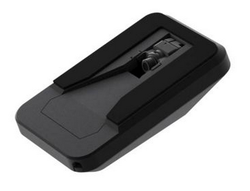
\includegraphics[scale=0.3]{mobileye}\label{fig:mobileye}}\hfill
    \subfloat[]{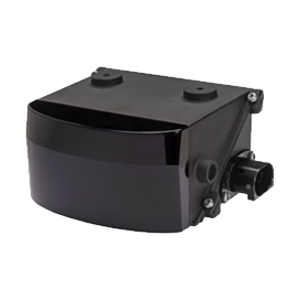
\includegraphics[scale=0.2]{SCALA_product_edit}\label{fig:scala}}\hfill
    \subfloat[]{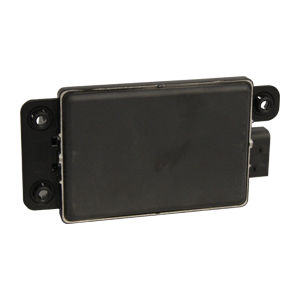
\includegraphics[scale=0.2]{delphi_esr_v2_300}\label{fig:delhi}}\\
    \subfloat[]{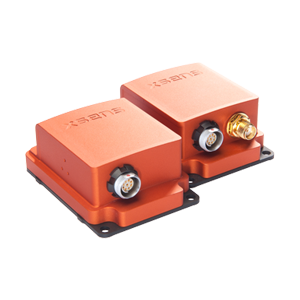
\includegraphics[scale=0.2]{MTi-100_productimg}\label{fig:mti-imu}}
    \hspace{2cm}
    \subfloat[]{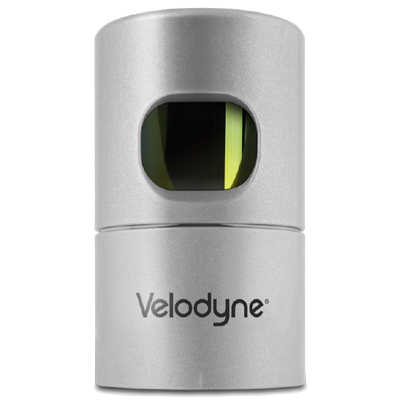
\includegraphics[scale=0.15]{HDL32E-for-web}\label{fig:hdl32}}
    \caption{Mia senses the environment with camera(a), lidar(b,e), radar(c) and imu-gps(d)  }
\end{figure}
\section{Vehicle Software}
In this section, we briefly explained what \acrshort{ros}. ROS is such an open-source operating system for robots that allows to run various executables in parallel and they are able to exchange their data and communicate between each other using a publish/subscribe messaging model.
ROS has three levels of concept but here we only discuss ROS Computation Graph Level and its basic concept including nodes, master, topics, and messages which are tools merely used in this project. We need these tools since communication is required between other subprojects’ nodes. These are the places which are performing the computation. For instance, one node can perform video stabilization, one can run extraction of railroad algorithm and another one can perform object detection then, publish their output. Moreover, a node can not only publish processing data but also can subscribe needed data from another node at the same time via a message which is a simple the data structure of ROS. By passing the message, allows nodes communicate with each other. The message can be thought as a bridge between nodes to provide an information flow. To access the information in the message, nodes use topics which navigate messages. The topic is used to determine the subject of the message. It means that one node publishes its data via message with a certain topic. One another node that is searching for particular data can acquire them with a specific topic as a subscriber. The roll of topic is to distinguish the information came from across nodes to prevent the wrong usage of information, because as mentioned before one node can publish and subscribe multi- message at the same time. Meanwhile, the topics allow nodes send or receive the message as long as they have appropriate topics. All these communication services are conducted by a master. The master allows ROS pieces to find and talk with each other.
